% -*- mode: latex; -*- mustache tags:  
\documentclass[10pt,twoside,english]{_support/latex/sbabook/sbabook}
\let\wholebook=\relax

\usepackage{import}
\subimport{_support/latex/}{common.tex}

%=================================================================
% Debug packages for page layout and overfull lines
% Remove the showtrims document option before printing
\ifshowtrims
  \usepackage{showframe}
  \usepackage[color=magenta,width=5mm]{_support/latex/overcolored}
\fi


% =================================================================
\title{The Pillar Super Book Archetype}
\author{The Pillar team}
\series{Square Bracket tutorials}

\hypersetup{
  pdftitle = {The Pillar Super Book Archetype},
  pdfauthor = {The Pillar team},
  pdfkeywords = {project template, Pillar, Pharo, Smalltalk}
}


% =================================================================
\begin{document}

% Title page and colophon on verso
\maketitle
\pagestyle{titlingpage}
\thispagestyle{titlingpage} % \pagestyle does not work on the first one…

\cleartoverso
{\small

  Copyright 2017 by The Pillar team.

  The contents of this book are protected under the Creative Commons
  Attribution-ShareAlike 3.0 Unported license.

  You are \textbf{free}:
  \begin{itemize}
  \item to \textbf{Share}: to copy, distribute and transmit the work,
  \item to \textbf{Remix}: to adapt the work,
  \end{itemize}

  Under the following conditions:
  \begin{description}
  \item[Attribution.] You must attribute the work in the manner specified by the
    author or licensor (but not in any way that suggests that they endorse you
    or your use of the work).
  \item[Share Alike.] If you alter, transform, or build upon this work, you may
    distribute the resulting work only under the same, similar or a compatible
    license.
  \end{description}

  For any reuse or distribution, you must make clear to others the
  license terms of this work. The best way to do this is with a link to
  this web page: \\
  \url{http://creativecommons.org/licenses/by-sa/3.0/}

  Any of the above conditions can be waived if you get permission from
  the copyright holder. Nothing in this license impairs or restricts the
  author's moral rights.

  \begin{center}
    
\includegraphics[width=0.2\textwidth]{_support/latex/sbabook/CreativeCommons-BY-SA.pdf}
  \end{center}

  Your fair dealing and other rights are in no way affected by the
  above. This is a human-readable summary of the Legal Code (the full
  license): \\
  \url{http://creativecommons.org/licenses/by-sa/3.0/legalcode}

  \vfill

  % Publication info would go here (publisher, ISBN, cover design…)
  Layout and typography based on the \textcode{sbabook} \LaTeX{} class by Damien
  Pollet.
}


\frontmatter
\pagestyle{plain}

\tableofcontents*
\clearpage\listoffigures

\mainmatter

\chapter{Lesson 15 –  Firmata implementation for the Pharo Programming Language.}
Firmata is a generic protocol for communicating with microcontrollers from software on a host computer. 
It is intended to work with any host computer software package. Right now there is a matching object in a number of languages. 
It is easy to add objects for other software to use this protocol. 
Basically, this firmware establishes a protocol for talking to the Arduino from the host software. 
The aim is to allow people to completely control the Arduino from software on the host computer.
\section{What do we need?}
In this lesson, we will use a setup with Pharo and Firmata.

\textbf{Components}

\begin{itemize}
\item 1 Arduino Uno
\item 1 Breadboard
\item 1 LED
\item 1 Resistor (330 ohms)
\item 1 Soil Moisture Sensor
\item Jumper wires
\end{itemize}
\section{Installation}\subsection{Arduino: Installing Standard Firmata}
\begin{itemize}
\item Your first step should be to download the Arduino application from 
\end{itemize}

\textbf{\href{https://www.arduino.cc/en/Main/Software}{Arduino Website.}\footnote{\url{https://www.arduino.cc/en/Main/Software}}} 

\begin{itemize}
\item Be sure to choose the latest version and also the correct download for your computer and operating system.
\item Once the software has downloaded, you can install the application using the method appropriate for your system. 
\end{itemize}

\begin{displaycode}{plain}
  -For Mac OS X you will be downloading a ZIP file. Double-clicking on the ZIP should produce a single "Arduino" application file which you can then copy into your Applications folder.
  -For Windows, you should download the .EXE containing a full Windows installer. Double clicking on the .EXE should start the installation.
  -For Linux you will download a compressed TAR file. You can use the "tar" command to uncompress and unpack the application.
\end{displaycode}

\begin{itemize}
\item Plug in Your Arduino Board as shown in Figure \ref{ArduinoConnection}.
\end{itemize}

\textbf{Note:} Disconnect any wires that may be attached to your Arduino and plug the board into the computer.

\begin{figure}

\begin{center}
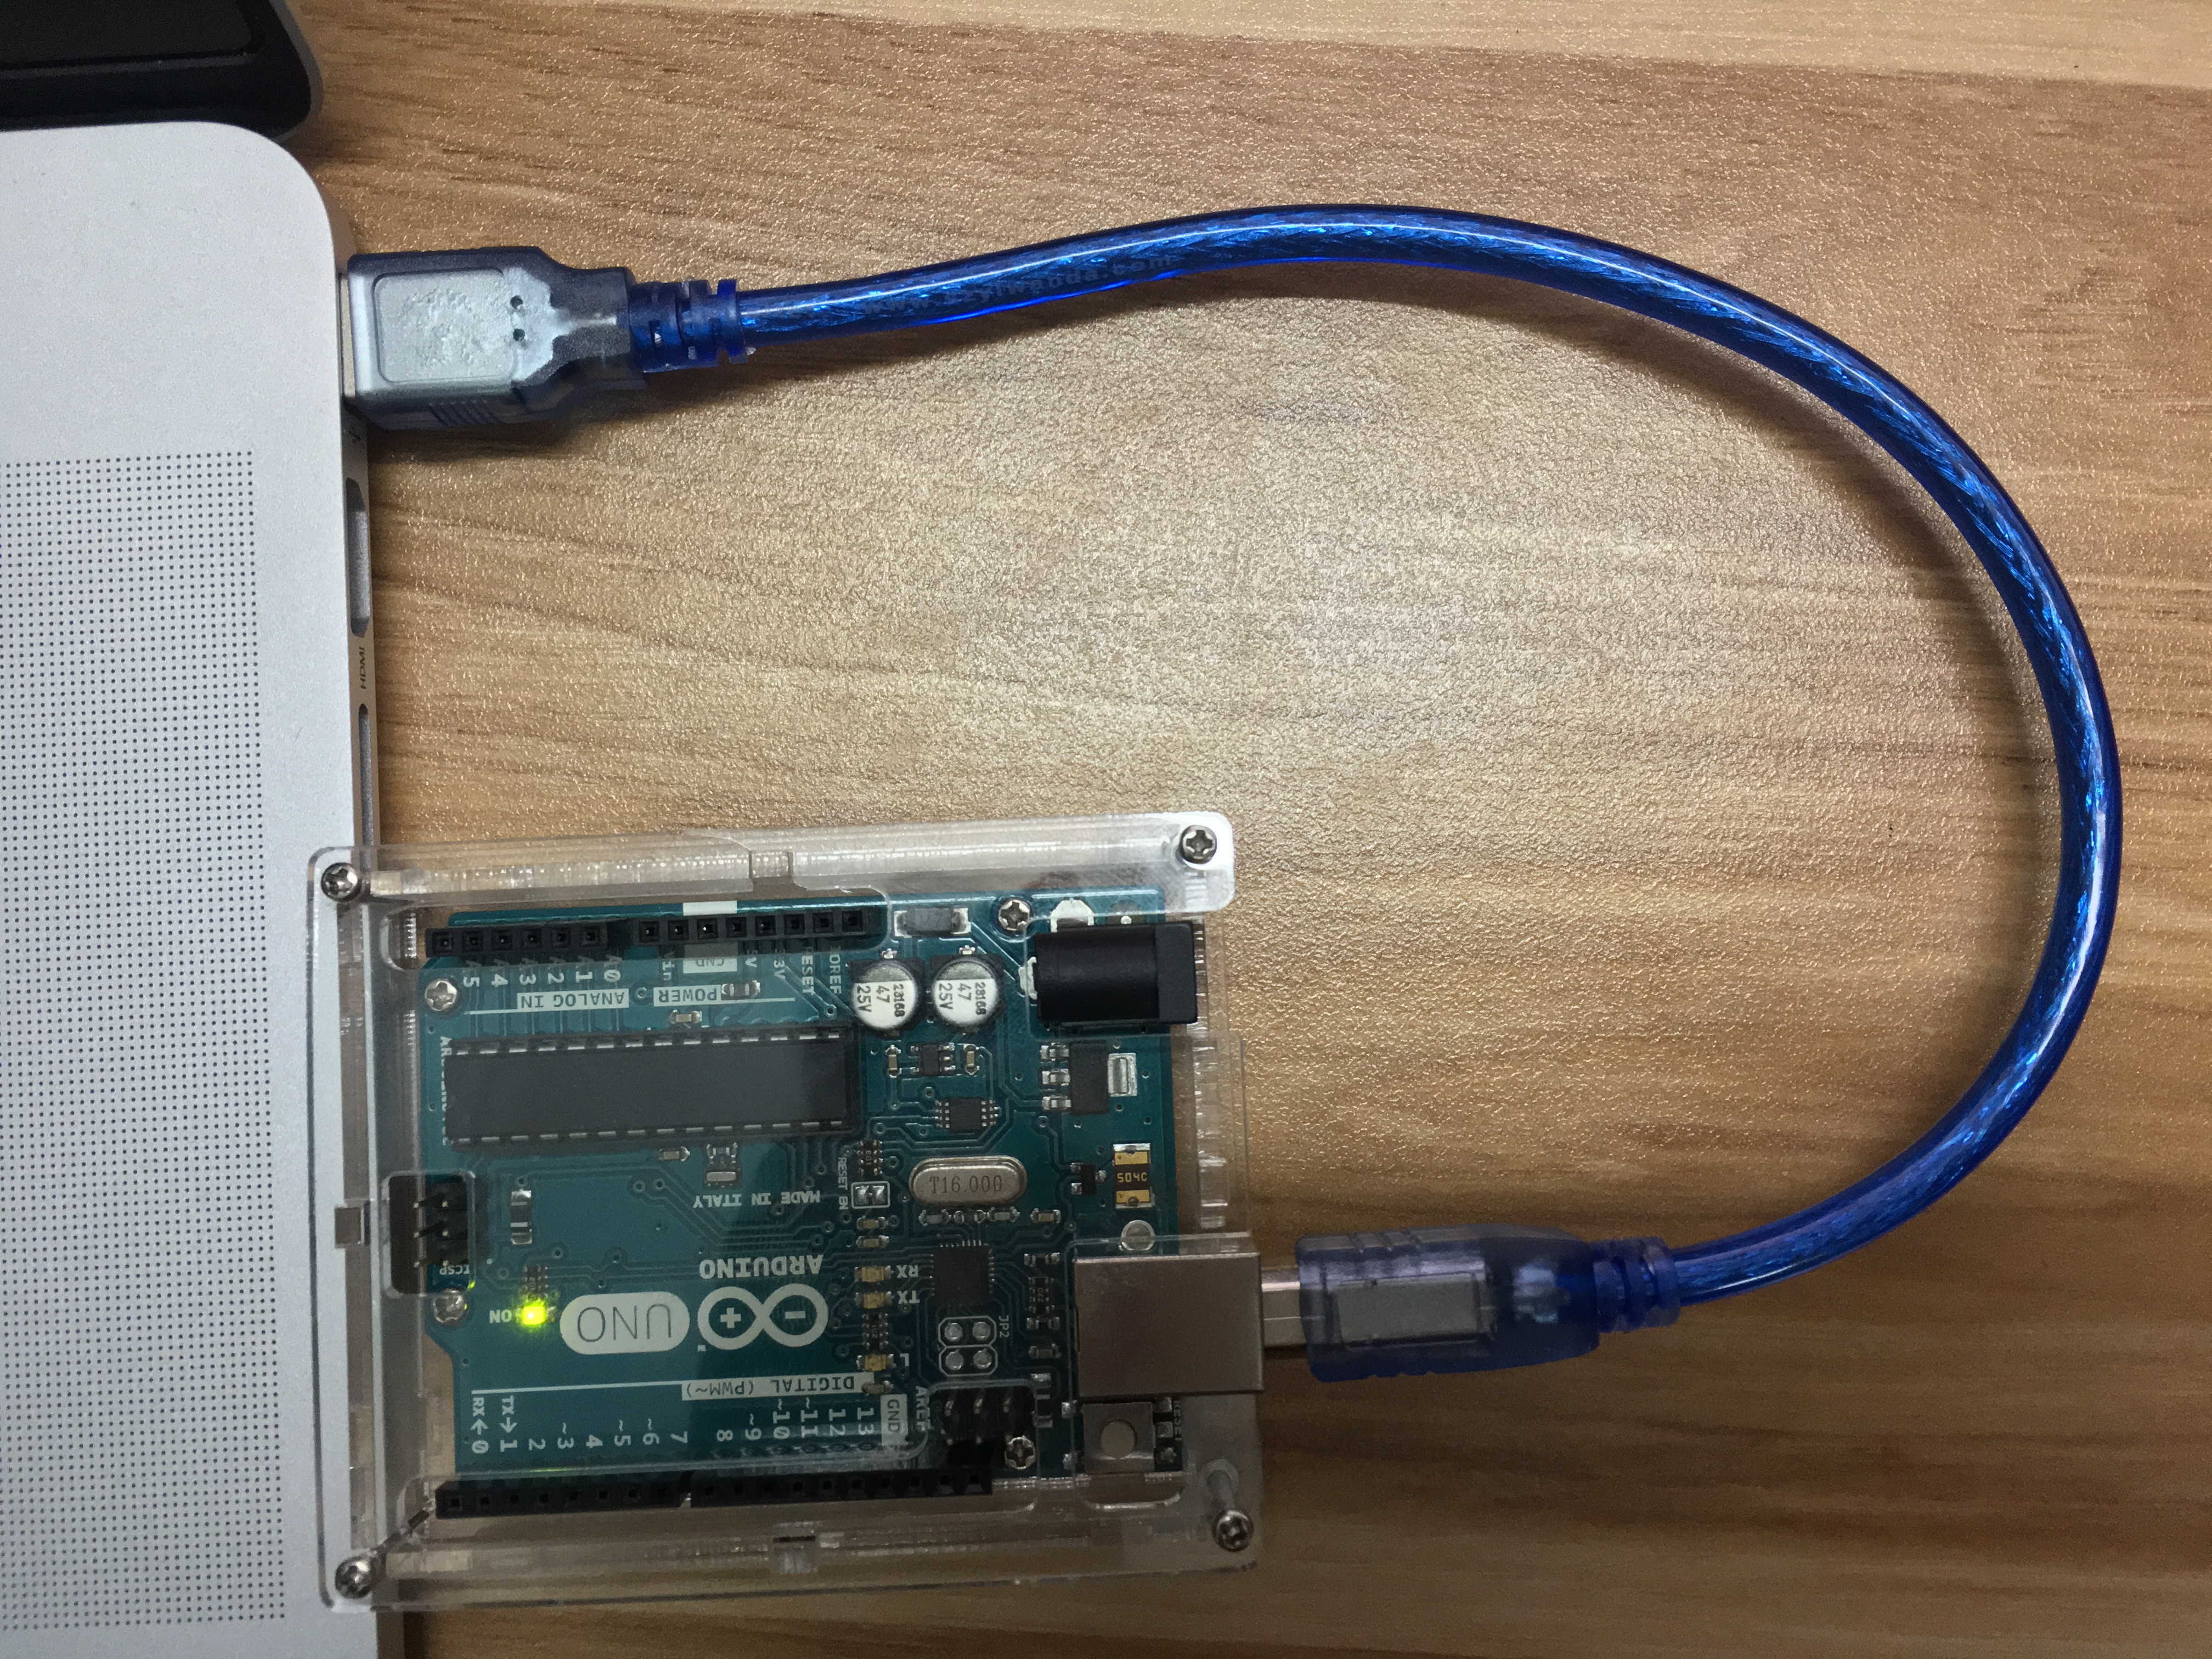
\includegraphics[width=0.7\textwidth]{/Users/kn/Chap14FirmataPharo/_result/pdf/Chapters/Chap14FirmataArduinoWithPharo/figures/IMG_3231.JPG}\caption{ArduinoUno.\label{ArduinoConnection}}\end{center}
\end{figure}


\begin{itemize}
\item You'll need to select the entry in the \textcode{Tools \textgreater{} Board menu} that corresponds to your Arduino board. 
\begin{itemize}
\item Here we are using Arduino UNO board and my port is \textcode{/dev/tty.usbmodem14201} ( You may have a different port name depend on your operating system ).
\end{itemize}

\item Upload the Standard Firmata Sketch
\end{itemize}


\begin{figure}

\begin{center}
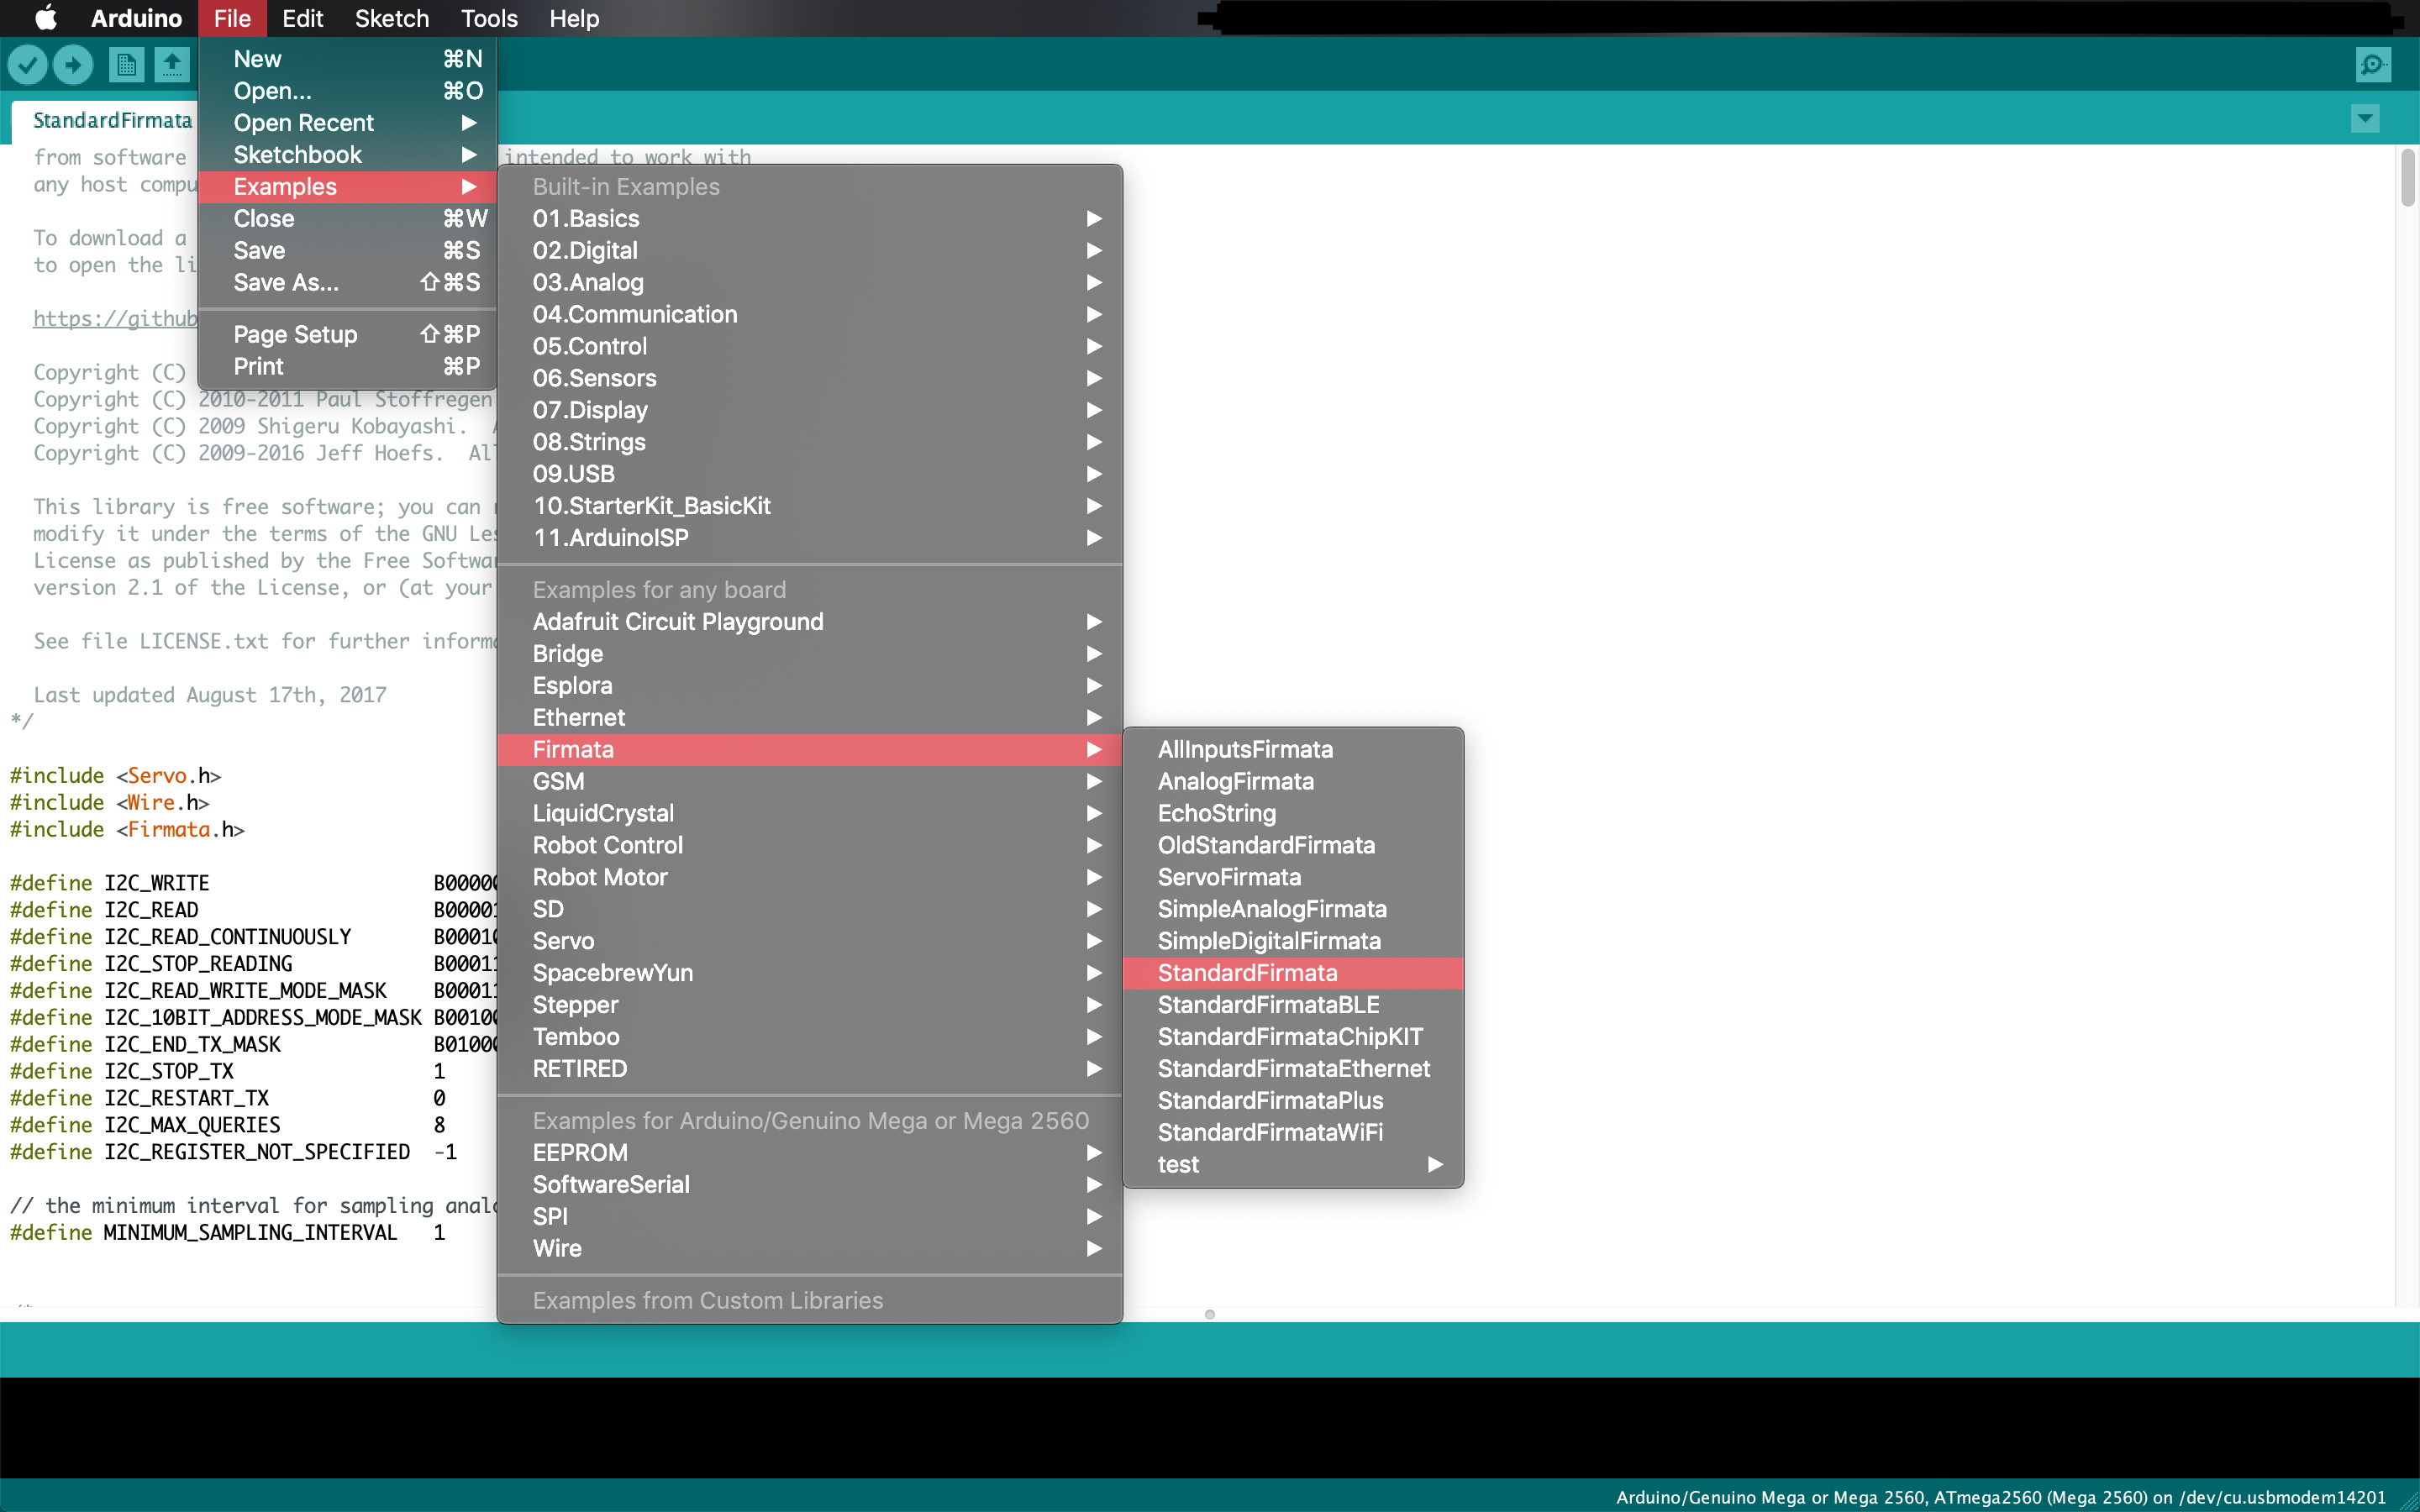
\includegraphics[width=0.7\textwidth]{/Users/kn/Chap14FirmataPharo/_result/pdf/Chapters/Chap14FirmataArduinoWithPharo/figures/firmataExample.JPG}\caption{Standard Firmata Example.\label{StandarFirmataExample}}\end{center}
\end{figure}


\begin{itemize}
\item 
\begin{itemize}
\item StandardFirmata is included with the Arduino IDE. To compile and upload StandardFirmata to your Arduino, open the IDE and select File/Examples/Firmata/StandardFirmata. 
\item Now at the top of the text editor window, click the \symbol{34}Upload\symbol{34} button on the IDE.
\item At the bottom of the text editor window, you should see a small status window. This will report the progress as the code is compiled and then uploaded to the Arduino. 
\item While the code is being uploaded, you should see some very small LED lights (the Transmit (TX) and Receive (RX) lights) on your Arduino board blinking as the data is transferred.
\item When the process is completed, you should see the message \symbol{34}Done Uploading\symbol{34} in the status window at the bottom of the editor.
\end{itemize}

\end{itemize}
\subsection{Pharo with Firmata}
To load latest version of Firmata you can evaluate the following expression in playground:

\begin{displaycode}{plain}
  Metacello new
  baseline: 'Firmata';
  repository: 'github://pharo-iot/Firmata';
  load
\end{displaycode}

We have tested this library so far with Arduino Uno and Funduino Uno. 
To connect to your firmatata enable device, you need the following things:

\begin{itemize}
\item Know the device's port name.
\item Know its baud rate.
\item Install firmata in it (you can do it using your arduino IDE).
\end{itemize}

For example, our Arduino boards use a baud rate of 57600, and were detected by our operating system in the /dev/ttyACM0 port. 
Connecting the Firmata client to arduino is as easy as follows:

\begin{displaycode}{plain}
  firmata := Firmata onPort: '/dev/ttyACM0' baudRate: 57600.
\end{displaycode}

Connecting to an arduino will check that the port exists, and will verify that Arduino has installed a compatible version of Firmata. 
In case one of these conditions does not hold, an exception is thrown.

Once we are connected, we can ask the Firmata driver if it is connected or not.

\begin{displaycode}{plain}
  firmata isConnected.
\end{displaycode}

And finally, we can disconnect it by doing:

\begin{displaycode}{plain}
  firmata disconnect.
\end{displaycode}
\section{Digital Pins}
The \textcode{digital inputs and outputs} (digital I/O) on the Arduino are what allow you to connect the Arduino sensors, actuators, and chips (intergrated circuit).
For example in Arduino UNO which is a microcontroller board based on the \symbol{34}ATmega328\symbol{34}. 
It has a few types of pins: \textbf{digital pin} ( 6 can be used as PWM outputs ), \textbf{analog pins} and orther pins like \textbf{power pins}

The \textcode{digital pins} on the Arduino can be configured as either inputs or outputs. 
There are only two state, either ON or OFF state and these states are represented by the binary values 1 and 0. 
You use digital signals in situations where the input or output will have one of those two values. 
In Arduino sketch terms, a ON state is known as HIGH (5V) and OFF state is known as LOW (0V). 
In other words, we can use them to obtain a digital value (for example, if a button is pressed or not), or to set a value (set if a led is turned on or off) but not both at the same time.
\subsection{Writing to Digital Pins}
To write to a digital pin, you should first set it to output mode using the \textcode{\#digitalPin:mode: message}. 
The first argument of the message is the number of the pin, and the second is a numeric value representing the output mode value. 
We use the \textcode{FirmataConstants} class that encapsulates many of the different numeric values used by firmata. 
In the following example, we set the digital pin 13 in output mode, so we can write to it.

\begin{displaycode}{plain}
  firmata digitalPin: 13 mode: FirmataConstants pinModeOutput.
\end{displaycode}

We can then write to a digital port with the \textcode{\#digitalWrite:value: message}, giving the pin number as first argument, and the value to write (0 or 1) as second argument. Thus, to turn on the pin 13 we can do:

\begin{displaycode}{plain}
  firmata digitalWrite: 13 value: 1.
\end{displaycode}

And to turn it off:

\begin{displaycode}{plain}
  firmata digitalWrite: 13 value: 0.
\end{displaycode}

You can use this method to toggle the LED as shown in Figure \ref{Controlling LED with Arduino via Digital pins}.

\begin{figure}

\begin{center}
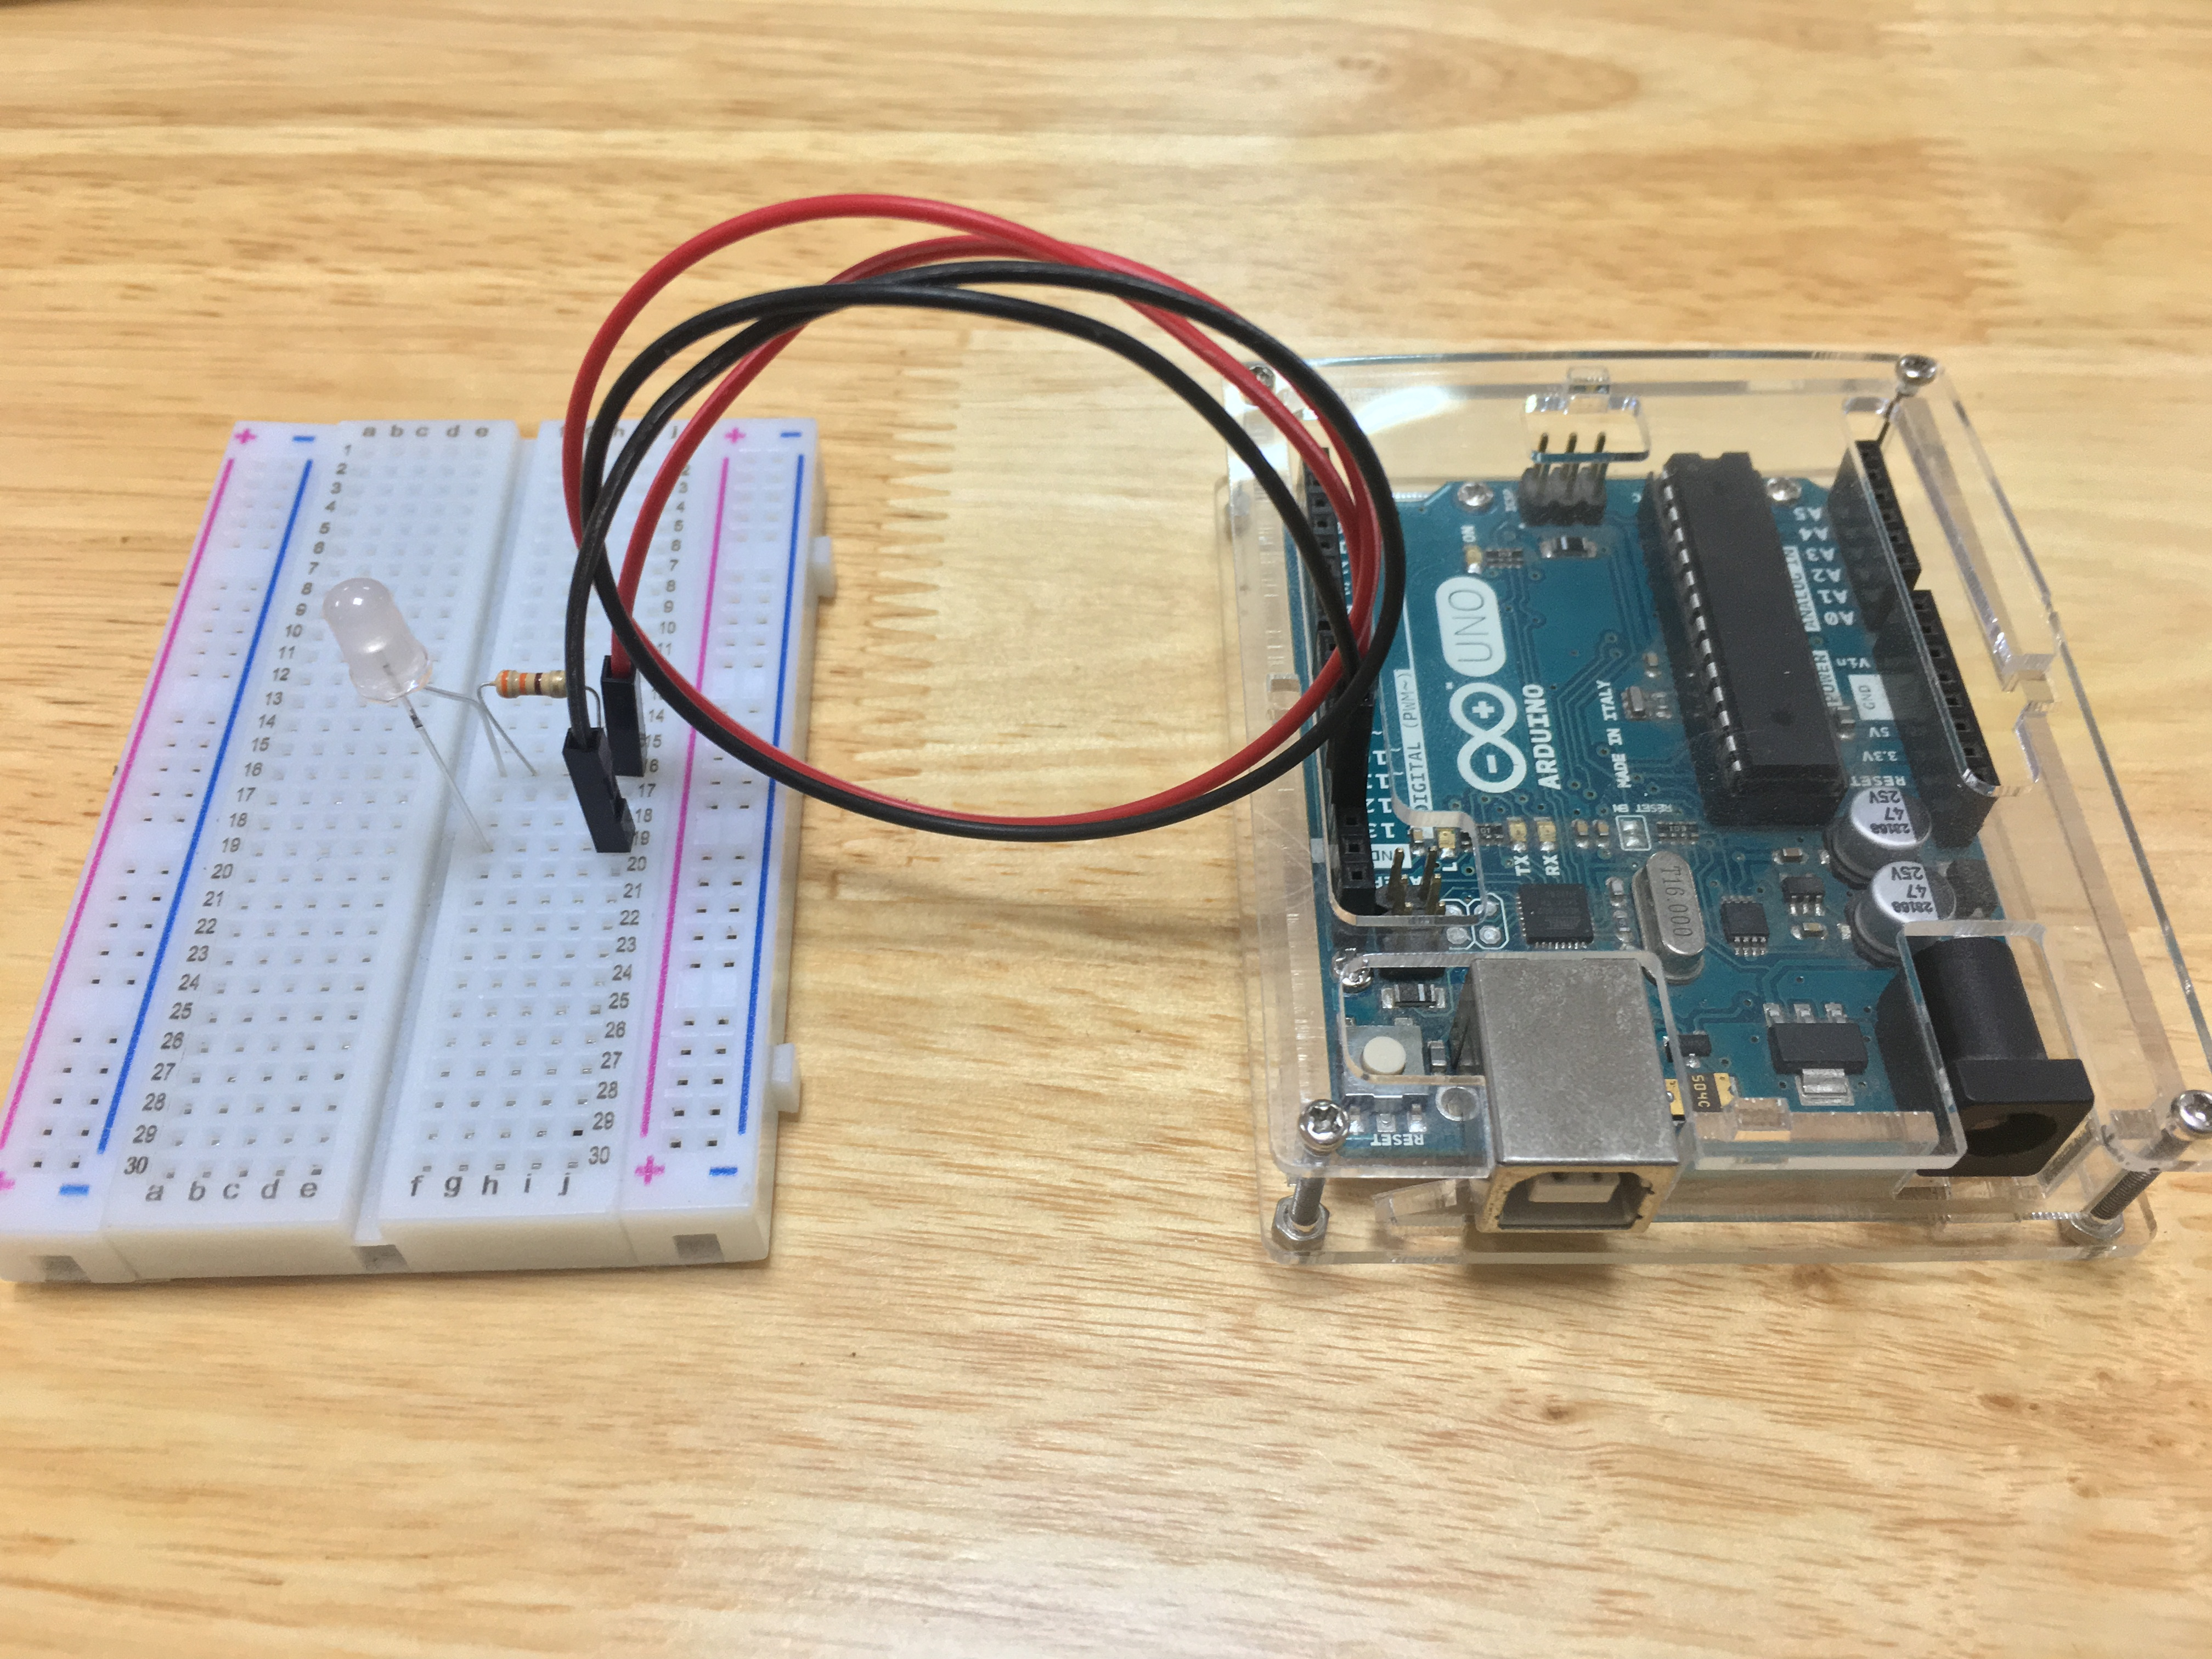
\includegraphics[width=0.7\textwidth]{/Users/kn/Chap14FirmataPharo/_result/pdf/Chapters/Chap14FirmataArduinoWithPharo/figures/IMG_3227.JPG}\caption{Controlling LED with Arduino via Digital pins.\label{Controlling LED with Arduino via Digital pins}}\end{center}
\end{figure}

\subsection{Reading from Digital Pins}
To read from a digital pin, you should first set it to input mode using the \textcode{\#digitalPin:mode: message}. 
The first argument of the message is the number of the pin, and the second is a numeric value representing the input mode value. 
We use the FirmataConstants class that encapsulates many of the different numeric values used by firmata.

In the following example, we first setup a push down button with a pull-down resistor.
We connect the button output to digital pin 2.
When we push the button and Firmata should tell us that the value of pin 2 is 1. When we do not push it, its value should be 0.


\begin{figure}

\begin{center}
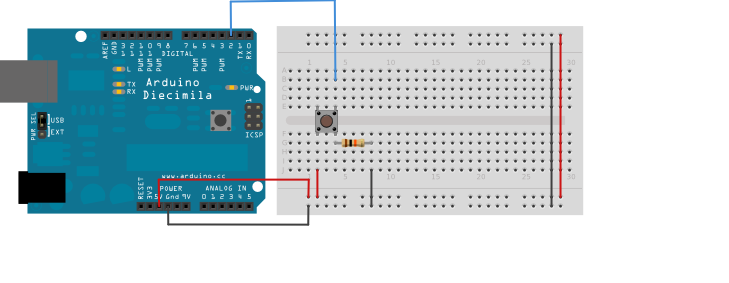
\includegraphics[width=0.9\textwidth]{/Users/kn/Chap14FirmataPharo/_result/pdf/Chapters/Chap14FirmataArduinoWithPharo/figures/digitalPinExample.jpg}\caption{Pull-down Resistor Button Sketch.\label{Pull-down Resistor Button Sketch}}\end{center}
\end{figure}


First, we set the digital pin 2 in input mode, so we can read from it.

\begin{displaycode}{plain}
  firmata digitalPin: 2 mode: FirmataConstants pinModeInput.
\end{displaycode}

Then, we can read the value of the pin using the \textcode{\#digitalRead:} message.

\begin{displaycode}{plain}
  firmata digitalRead: 2.
\end{displaycode}

If we ask the value and press the button at the same time, we get the value 1.
\section{Analog Pins}
Analog pins are pins whose state range in the continuum between 0 and 1. These states are represented as floating point numbers.

As with digital pins, analog pins work both in read and write mode. 
Typical usages of reading analog pins is retrieving data from sensors, such as temperature, humidity, light and so on. 
Writing analog pins can be used to, for example, turn on leds with a given intensity instead of just \symbol{34}turning on\symbol{34} like we do with the digital pins.
\subsection{Activating Analog Pins}
\begin{displaycode}{plain}
  firmata activateAnalogPin: 0.
\end{displaycode}
\subsection{Reading from Analog Pins}
\begin{displaycode}{plain}
  ((firmata analogRead: 0) * 500 / 1024) asFloat.
\end{displaycode}
\section{Experimental procedure}
The Soil Moisture Sensor measures soil moisture grace to the changes in electrical conductivity of the earth ( soil resistance increases with drought ).
The electrical resistance is measured between the two electrodes of the sensor.
A comparator activates a digital output when a adjutable threshold is exceeded.
There are a lot of moisture sensors but in our example, we use the Capacitive Soil Moisture Sensor from DFTrobot as the figure \ref{Capacitive-Soil-Moisture Sensor}

\begin{figure}

\begin{center}
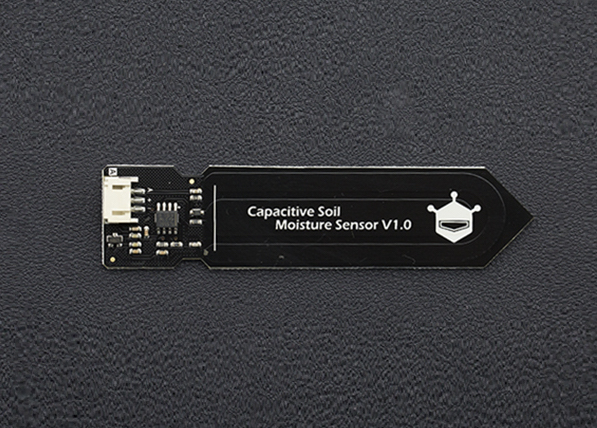
\includegraphics[width=0.6\textwidth]{/Users/kn/Chap14FirmataPharo/_result/pdf/Chapters/Chap14FirmataArduinoWithPharo/figures/SEN0193.jpg}\caption{Capacitive-Soil-Moisture Sensor.\label{Capacitive-Soil-Moisture Sensor}}\end{center}
\end{figure}


The Figure \ref{Capacitive-Soil-Moisture Sensor Sketch} shows how the electric connection is made.


\begin{figure}

\begin{center}
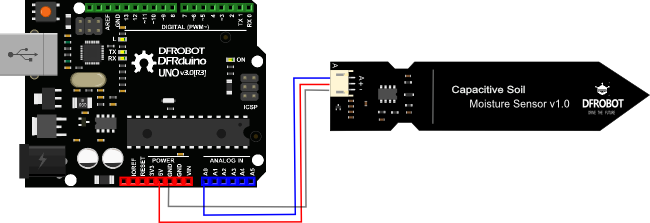
\includegraphics[width=0.9\textwidth]{/Users/kn/Chap14FirmataPharo/_result/pdf/Chapters/Chap14FirmataArduinoWithPharo/figures/capacitiveSoilMoistureSensor.png}\caption{Capacitive-Soil-Moisture Sensor Sketch.\label{Capacitive-Soil-Moisture Sensor Sketch}}\end{center}
\end{figure}


\begin{tabular}{ll}
\toprule
\textbf{Aduino Uno} & \textbf{Capacitive Soil Moisture Sensor} \\
\midrule
GND & Black wire \\
5V & Red Wire \\
Analog output & Blue Wire \\
\bottomrule
\end{tabular}
\subsection{Connecting the Firmata client to arduino}
\begin{displaycode}{plain}
  firmata := Firmata onPort: '/dev/ttyACM0' baudRate: 57600.
\end{displaycode}
\subsection{Check the firmata connection}
\begin{displaycode}{plain}
  firmata isConnected.
\end{displaycode}
\subsection{Getting the temperature with Capacitive-Soil-Moisture Sensor}
\begin{displaycode}{plain}
  firmata activateAnalogPin: 0.
  firmata analogRead:0.
\end{displaycode}
\subsection{Result }
This is very simple and you can get these values and stored in a variable, to use to different purposes, like send a message to an LCD display, send the values to a cloud server and simply do some action.


\begin{figure}

\begin{center}
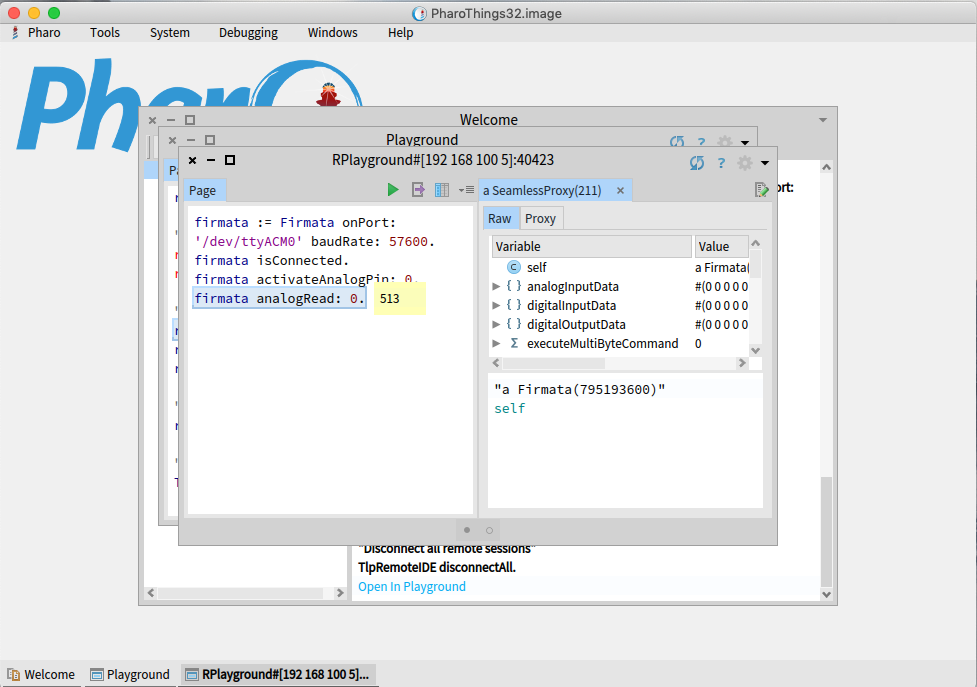
\includegraphics[width=0.9\textwidth]{/Users/kn/Chap14FirmataPharo/_result/pdf/Chapters/Chap14FirmataArduinoWithPharo/figures/result.png}\caption{Capacitive-Soil-Moisture Sensor with Arduino via Firmata Result.\label{Capacitive-Soil-Moisture Sensor with Arduino via Firmata Result}}\end{center}
\end{figure}




\bibliographystyle{alpha}
\bibliography{book.bib}

% lulu requires an empty page at the end. That's why I'm using
% \backmatter here.
\backmatter

% Index would go here

\end{document}
